\documentclass[xcolor=table,aspectratio=169]{beamer}
\usetheme{Madrid}
\beamertemplatenavigationsymbolsempty
\usepackage{graphicx}
\usepackage[table]{xcolor}
\usepackage[most, skins]{tcolorbox}
\usepackage{helvet}
% Definitions of colours used in seaborn for use in latex
\definecolor{seaborn_bg_grey}{HTML}{eaeaf2}
\definecolor{seaborn_bg_grey_dark}{HTML}{d2d2d9}
\definecolor{seaborn_bg_grey_darker}{HTML}{a3a3a9}
\definecolor{seaborn_bg_grey_half}{HTML}{f4f4f8}

\definecolor{seaborn_blue}{HTML}{4c72b0}
\definecolor{seaborn_orange}{HTML}{da8558}
\definecolor{seaborn_green}{HTML}{55a868}
\definecolor{seaborn_red}{HTML}{c44e52}
\definecolor{seaborn_magenta}{HTML}{8172b2}
\definecolor{seaborn_yellow}{HTML}{ccb974}
\definecolor{seaborn_cyan}{HTML}{64b5cd}

\definecolor{seaborn_muted_blue}{HTML}{4878cf}
\definecolor{seaborn_muted_green}{HTML}{6acc65}
\definecolor{seaborn_muted_red}{HTML}{d65f5f}
\definecolor{seaborn_muted_magenta}{HTML}{b47cc7}
\definecolor{seaborn_muted_yellow}{HTML}{c4ad66}
\definecolor{seaborn_muted_cyan}{HTML}{77bedb}

\definecolor{seaborn_pastel_blue}{HTML}{92c6ff}
\definecolor{seaborn_pastel_green}{HTML}{97f0aa}
\definecolor{seaborn_pastel_red}{HTML}{ff9f9a}
\definecolor{seaborn_pastel_magenta}{HTML}{d0bbff}
\definecolor{seaborn_pastel_yellow}{HTML}{fffea3}
\definecolor{seaborn_pastel_cyan}{HTML}{b0e0e6}

\definecolor{seaborn_bright_blue}{HTML}{003fff}
\definecolor{seaborn_bright_green}{HTML}{03ed3a}
\definecolor{seaborn_bright_red}{HTML}{e8000b}
\definecolor{seaborn_bright_magenta}{HTML}{8a2be2}
\definecolor{seaborn_bright_yellow}{HTML}{ffc400}
\definecolor{seaborn_bright_cyan}{HTML}{00d7ff}

\definecolor{seaborn_dark_blue}{HTML}{001c7f}
\definecolor{seaborn_dark_green}{HTML}{017517}
\definecolor{seaborn_dark_red}{HTML}{8c0900}
\definecolor{seaborn_dark_magenta}{HTML}{7600a1}
\definecolor{seaborn_dark_yellow}{HTML}{b8860b}
\definecolor{seaborn_dark_cyan}{HTML}{006374}

\definecolor{seaborn_colorblind_blue}{HTML}{0072b2}
\definecolor{seaborn_colorblind_green}{HTML}{009e73}
\definecolor{seaborn_colorblind_red}{HTML}{d55e00}
\definecolor{seaborn_colorblind_magenta}{HTML}{cc79a7}
\definecolor{seaborn_colorblind_yellow}{HTML}{f0e442}
\definecolor{seaborn_colorblind_cyan}{HTML}{56b4e9}


\usepackage{adjustbox}

% Tikz
\usepackage{tikz}
\usetikzlibrary{positioning,shapes,arrows,backgrounds,fit,calc,external}
\tikzexternalize
\tikzstyle{dummy} = []
\tikzstyle{line} = [draw, thick, -latex']
\tikzstyle{headless_line} = [draw, thick, -]
\tikzstyle{default}    = [rectangle, text centered, rounded corners, text=black, font=\sffamily\footnotesize, align=center]
\tikzstyle{default_text}    = [rectangle, text width=10cm, text=black,anchor=north west, font=\sffamily]
\tikzstyle{boxwhite} = [default, fill=white, rounded corners=0.1cm]
\tikzstyle{cp}    = [default, fill=seaborn_blue, text=white, text width=2.8cm, minimum height=0.5cm]
\tikzstyle{pw}    = [cp, fill=seaborn_green]
\tikzstyle{wannier90}    = [cp, fill=seaborn_cyan]
\tikzstyle{bespoke}    = [cp, fill=seaborn_magenta]
\tikzstyle{observable}    = [cp, fill=seaborn_red]
\tikzset{
  -|-/.style={
    to path={
      (\tikztostart) -| ($(\tikztostart)!#1!(\tikztotarget)$) |- (\tikztotarget)
      \tikztonodes
    }
  },
  -|-/.default=0.5,
  |-|/.style={
    to path={
      (\tikztostart) |- ($(\tikztostart)!#1!(\tikztotarget)$) -| (\tikztotarget)
      \tikztonodes
    }
  },
  |-|/.default=0.5,
}

\newlength{\myyshift}
\setlength{\myyshift}{0.05cm}

\definecolor{darkblue}{HTML}{315472}
\setbeamercolor{frametitle}{bg=black, fg=white}
\setbeamercolor{body}{fg=black, bg=white}
\setbeamercolor*{author in head/foot}{bg=darkblue}
\setbeamercolor*{logo in head/foot}{bg=darkblue,fg=white}
\setbeamercolor*{title in head/foot}{bg=darkblue,fg=white}
\setbeamercolor*{date in head/foot}{bg=darkblue,fg=white}
\setbeamercolor{title}{bg=darkblue}
\setbeamercolor{footline}{bg=darkblue}
\setbeamercolor{caption name}{fg=darkblue}
\setbeamersize{text margin left=0.07cm,text margin right=0.07cm}
\setbeamercolor{background canvas}{bg=seaborn_bg_grey_dark}

% New commands
\newcommand{\ket}[1]{|#1\rangle}
\newcommand{\bra}[1]{\langle #1|}
\newcommand{\braket}[2]{\langle #1|#2\rangle}
\newcommand{\braopket}[3]{\langle #1|#2|#3\rangle}
\newcommand{\nline}{\nonumber \\}
\newcommand{\Trace}{\mathrm{Tr}}

\setbeamertemplate{frametitle}
{
  \vspace{-1pt}
  \begin{beamercolorbox}[wd=\paperwidth,ht=0.8cm]{frametitle}
    \hspace{0.05em}
    \begin{minipage}{0.85\textwidth}
      \small \bf
      Accurately predicting electron affinities with Koopmans spectral functionals

      \tiny
      Edward Linscott, Nicola Colonna, Riccardo De Gennaro, and Nicola Marzari
    \end{minipage}
    \hfill
    \begin{minipage}{0.1\textwidth}
    \includegraphics[height=0.55cm]{/home/elinscott/Pictures/epfl_logos/white_cropped.eps}
    \end{minipage}
    \hspace{0.2cm}
    \vspace{0.125cm}
  \end{beamercolorbox}%
}
\setbeamertemplate{title page}
{
}
%\setbeamerfont{frametitle}{series=\bfseries}
\setbeamertemplate{footline}{}

\begin{document}

\begin{frame}{x}
  \hbox{
    \begin{beamercolorbox}[wd=0.3\textwidth,ht=0.89\textheight,sep=0.1cm]{body}
      \footnotesize \textbf{Theory}

      \vspace{1.4ex}

      \centering

      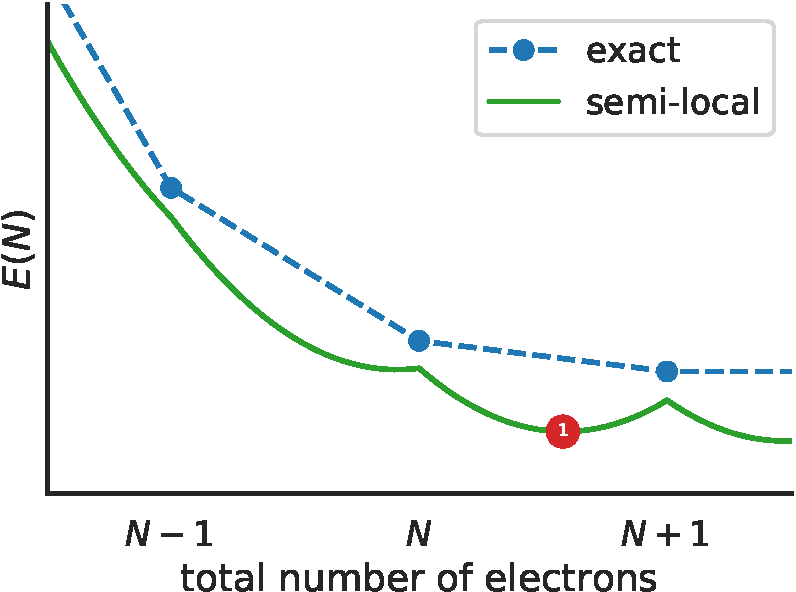
\includegraphics[width=0.2\columnwidth]{../figures/curvature_plot/fig_en_curve_koopmans_step1-crop.pdf}

      %
      \tiny The goal:

      $\varepsilon_i = \braopket{\varphi_i}{H}{\varphi_i} = \partial E/\partial f_i$ independent of $f_i$

      \vspace{2em}

      The functional:
      %
      \begin{align*}
         & E_{KC}[\rho,\{f_i\},\{\alpha_i\}] = \only<1>{\textcolor{seaborn_bright_red}}{E_{DFT}[\rho]} \nonumber \\
         & + \sum_i \alpha_i\left(
        \only<2>{\textcolor{seaborn_bright_red}}{- \int^{f_i}_{0} \varepsilon_i(f) df}
        \only<3>{\textcolor{seaborn_bright_red}}{\, + f_i \int_0^1 \varepsilon_i(f) df}
        \right)
      \end{align*}

      \textcolor{seaborn_bg_grey_dark}{Dabo \emph{et al}, Phys. Rev. B 82, 115121}

      \textcolor{seaborn_bg_grey_dark}{Borghi \emph{et al}, Phys. Rev. B 90, 075135}

      \textcolor{seaborn_bg_grey_dark}{Nguyen \emph{et al}, Phys. Rev. X 8, 021051}
    \end{beamercolorbox}%
    \hspace{0.01\textwidth}%
    \vbox{

      \begin{beamercolorbox}[wd=0.6775\textwidth,ht=0.52\textheight,sep=0.1cm]{body}
        \footnotesize \textbf{Implementation}
        \tiny
      \end{beamercolorbox}%
      \vspace{0.7ex}

      \begin{beamercolorbox}[wd=0.6775\textwidth,ht=0.35\textheight,sep=0.1cm]{body}
        \footnotesize \textbf{Results}
        \vspace{0.2em}

        % \begin{tabular}{c c}
        %   \includegraphics[height=0.23\textheight]{../figures/gw100_ips.jpeg}
        %    &
        %   \includegraphics[height=0.23\textheight]{../figures/fig_gw100_ea_mae_mse-crop.pdf}
        %   \\
        %   \tiny \textcolor{seaborn_bg_grey_dark}{Colonna \emph{et al}, JCTC 2018, 14, 5, 2549–2557}
        %    &
        %   \tiny \textcolor{seaborn_bg_grey_dark}{Linscott \emph{et al}, in prep.}
        % \end{tabular}
      \end{beamercolorbox}
    }%
  }
\end{frame}

\end{document}
